\question{Приложения определенного интеграла: вычисление площади криволинейного сектора в полярных координатах.}

\begin{minipage}{\linewidth}
  \begin{multicols*}{2}
  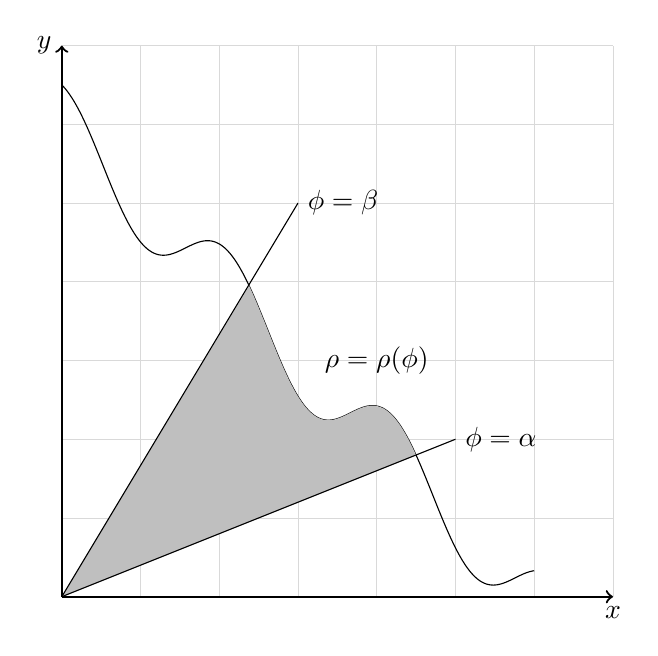
\begin{tikzpicture}

    \draw[very thin, gray!30, step = 1cm] (0, 0) grid (7, 7);
    \draw[domain = 0 : 6, variable = \x, samples = 5000]
      plot ({\x}, {6 - \x + 0.5 * cos(deg(3 * \x))});
    \fill[lightgray, domain = 2.38 : 4.5, variable = \x, samples = 5000]
      (0, 0)
       -- plot ({\x}, {6 - \x + 0.5 * cos(deg(3 * \x))})
       -- cycle;

    \draw (0, 0) -- (5, 2) node[right] {\(\phi = \alpha\)};
    \draw (0, 0) -- (3, 5) node[right] {\(\phi = \beta\)};
    \draw node at (4, 3) {\(\rho = \rho(\phi)\)};

    \draw[thick] [->] (0, 0) -- (7, 0) node[right, below] {\(x\)};
    \draw[thick] [->] (0, 0) -- (0, 7) node[above, left] {\(y\)};
  \end{tikzpicture}
  \columnbreak

  Построим интеграл:
  \begin{enumerate}
    \item Дробление отрезка \([\alpha, \beta]\) на подотрезки
      \([\phi_{i - 1}, \phi_{i}]\), \(\tau = \max \Delta \phi_{i}\).

    \item В каждом отрезке выбираем среднюю точку \(\xi_{i}\). Ищем
      \(\rho(\xi_{i})\), приближаем площадь элементарного сектора площадью
      кругового.
    
      \begin{align*}
        S_{sec}
        = \frac{\pi \rho^2(\xi_{i})}{2 \pi} \cdot \Delta \phi_{i}
        = \frac{1}{2} \rho^2(\xi_{i}) \Delta \phi_{i}
      \end{align*}

    \item Площадь это предел интегральных сумм
    
    \begin{align*}
      S = \lim_{\substack{n \to \infty \\ \tau \to 0}}
        \sum_{i = 1}^{n} \frac{1}{2} \rho^2(\xi_{i}) \Delta \phi_{i}
    \end{align*}
    
    \item Переход к интегралу
    \begin{align*}
      S = \frac{1}{2} \int_{\alpha}^{\beta} \rho^2(\phi) \dd \phi
    \end{align*}
  \end{enumerate}

  \end{multicols*}
\end{minipage}